\chapter{Classification} \label{Classification}


\begin{enumerate}
    \item machine learning practitioners overload the word classification to describe two subtly different problems: \cite{d2l}

    \begin{enumerate}
        \item those where we are interested only in \textbf{hard assignments} of examples to categories (classes);
        
        \item those where we wish to make \textbf{soft assignments}, i.e., to assess the \textbf{probability} that each category applies. 

    \end{enumerate}

    \item The distinction tends to get blurred, in part, because often, even when we only care about hard assignments, we still use models that make soft assignments. \cite{d2l}

    \item There are cases where more than one label might be true. For instance, a news article might simultaneously cover the topics of entertainment, business, and space flight, but not the topics of medicine or sports. Thus, categorizing it into one of the above categories on their own would not be very useful. This problem is commonly known as \textbf{multi-label classification}\indexlabel{multi-label classification} \cite{d2l}

    \item If the categories had some natural ordering among them, say if we were trying to predict $\{\textrm{baby}, \textrm{toddler}, \textrm{adolescent}, \textrm{young adult}, \textrm{adult}, \textrm{geriatric}\}$, then it might even make sense to cast this as an \textbf{ordinal regression}\indexlabel{ordinal regression} problem and keep the labels in this format.
\end{enumerate}


\section{Softmax Regression \cite{dnn-1}} \label{classification: Softmax Regression}

SEE: 
\begin{enumerate}
    \item \fullref{Softmax function}
\end{enumerate}

\subsection{Linear Model \cite{dnn-1}} \label{classification: Softmax Regression: Linear Model}

\begin{enumerate}[itemsep=0.2cm]
    \item In order to estimate the \textbf{conditional probabilities} associated with all the possible classes, we need a model with \textbf{multiple outputs}, one per class. 
    
    \item To address classification with linear models, we will need as many \textbf{affine functions} as we have outputs. 
    
    \item Strictly speaking, we only need \textbf{one fewer}, since the final category has to be the difference between $1$ and the sum of the other categories, but for reasons of \textbf{symmetry} we use a slightly \textbf{redundant parametrization}. 
    
    \item Each output corresponds to its own affine function. 
    
    \item For example, if we have $4$ \textbf{features} and $3$ possible \textbf{output} categories, we need $12$ scalars to represent the \textbf{weights} ($w$ with subscripts), and $3$ scalars to represent the biases ($b$ with subscripts). 
    
    \item This yields:
    \begin{table}[H]
        \begin{minipage}{0.49\linewidth}
            \begin{figure}[H]
                \centering
                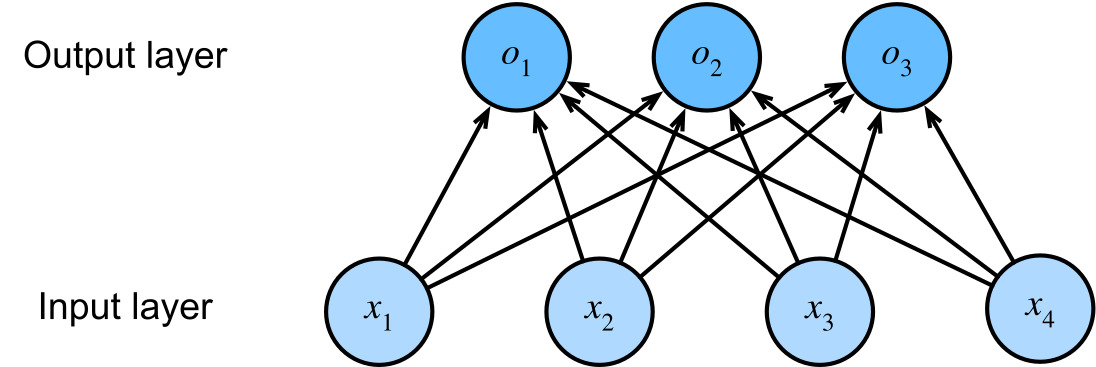
\includegraphics[width=\linewidth, height=2.5cm, keepaspectratio]{Pictures/deep_neural_networks/softmaxreg-4.1.1.jpg}
            \end{figure}
        \end{minipage}
        \hfill
        \begin{minipage}{0.49\linewidth}
            \[
                \begin{aligned}
                    o_1 &= x_1 w_{11} + x_2 w_{12} + x_3 w_{13} + x_4 w_{14} + b_1\\
                    o_2 &= x_1 w_{21} + x_2 w_{22} + x_3 w_{23} + x_4 w_{24} + b_2\\
                    o_3 &= x_1 w_{31} + x_2 w_{32} + x_3 w_{33} + x_4 w_{34} + b_3
                \end{aligned}
            \]
            \[ \mathbf{o} = \mathbf{W} \mathbf{x} + \mathbf{b} \]
        \end{minipage}
    \end{table}
    

    \item Just as in linear regression, we use a \textbf{single-layer neural network}. 
    
    \item And since the calculation of each output, $o_1, o_2$, and $o_3$, depends on all inputs, $x_1, x_2, x_3,$ and $x_4$, the output layer can also be described as a \textbf{fully connected layer}.

\end{enumerate}



\subsection*{Using Softmax}

\begin{enumerate}[itemsep=0.2cm]
    \item Assuming a suitable loss function, we could try, directly, to minimize the difference between $o$ and the labels $y$.

    \item While it turns out that treating classification as a vector-valued regression problem works surprisingly well, it is nonetheless lacking in the following ways:
    \begin{enumerate}
        \item There is no guarantee that the outputs $o_i$ sum up to $1$ in the way we expect probabilities to behave.

        \item There is no guarantee that the outputs oi are even non-negative, even if their outputs sum up to $1$, or that they do not exceed $1$.

    \end{enumerate}

    \item Both aspects render the estimation problem difficult to solve and the solution very brittle to outliers.

\end{enumerate}










































